
\documentclass{beamer}
\usetheme{CambridgeUS}

\setbeamertemplate{caption}[numbered]{}

\usepackage{enumitem}
\usepackage{tfrupee}
\usepackage{amsmath}
\usepackage{amssymb}
\usepackage{textcomp, gensymb}
\usepackage{graphicx}
\usepackage{txfonts}
                               
\providecommand{\pr}[1]{\ensuremath{\Pr\left(#1\right)}}
\providecommand{\mbf}{\mathbf}
\providecommand{\qfunc}[1]{\ensuremath{Q\left(#1\right)}}
\providecommand{\sbrak}[1]{\ensuremath{{}\left[#1\right]}}
\providecommand{\lsbrak}[1]{\ensuremath{{}\left[#1\right.}}
\providecommand{\rsbrak}[1]{\ensuremath{{}\left.#1\right]}}
\providecommand{\brak}[1]{\ensuremath{\left(#1\right)}}
\providecommand{\lbrak}[1]{\ensuremath{\left(#1\right.}}
\providecommand{\rbrak}[1]{\ensuremath{\left.#1\right)}}
\providecommand{\cbrak}[1]{\ensuremath{\left\{#1\right\}}}
\providecommand{\lcbrak}[1]{\ensuremath{\left\{#1\right.}}
\providecommand{\rcbrak}[1]{\ensuremath{\left.#1\right\}}}
\providecommand{\abs}[1]{\vert#1\vert}
\newcommand*{\permcomb}[4][0mu]{{{}^{#3}\mkern#1#2_{#4}}}
\newcommand*{\perm}[1][-3mu]{\permcomb[#1]{P}}
\newcommand*{\comb}[1][-1mu]{\permcomb[#1]{C}}

\newcounter{saveenumi}
\newcommand{\seti}{\setcounter{saveenumi}{\value{enumi}}}
\newcommand{\conti}{\setcounter{enumi}{\value{saveenumi}}}

\makeatletter
\newenvironment<>{proofs}[1][\proofname]{%
    \par
    \def\insertproofname{#1\@addpunct{.}}%
    \usebeamertemplate{proof begin}#2}
  {\usebeamertemplate{proof end}}
\makeatother

\title{Assignment 3}
\author{JARUPULA SAI KUMAR (CS21BTECH11023)}
\date{\today}
\logo{\large \LaTeX{}}


\begin{document}

% Title page frame
\begin{frame}
    \titlepage 
\end{frame}

% Remove logo from the next slides
\logo{}


% Outline frame
\begin{frame}{Outline}
    \tableofcontents
\end{frame}

%Question
\section{Question}
\textbf{QUESTION 4.13 :}
\textbf{QUESTION 4.13 :}
A fair coin is tossed three times and the random variable x equals the total number of heads.
Find and sketch $F_x(x)$ and $f_x(x)$.
\textbf{Solution :}
let x be a random variable which maps to 1 when coin denotes head and 0 when it denotes tail.
\begin{table}[ht!]
		\centering
	
		\caption{Events and Description}
		\label{table:1}
\end{table}
 probability of getting r heads is $\pr{X=k} = \binom{n}{k}\times p^k \times (1-p)^k$
 so 
 \begin{align}
     &\pr{X=0} = \binom{3}{0}\times \frac{1}{2}^0 \times (1-\frac{1}{2})^3 = \frac{1}{8}& \\
 &\pr{X=1} = \binom{3}{1}\times \frac{1}{2}^1 \times (1-\frac{1}{2})^2 = \frac{3}{8}& \\   
 &\pr{X=2} = \binom{3}{2}\times \frac{1}{2}^2 \times (1-\frac{1}{2})^1 = \frac{3}{8}& \\
 &\pr{X=3} = \binom{3}{3}\times \frac{1}{2}^3 \times (1-\frac{1}{2})^0 = \frac{1}{8}& 
 \end{align}
 
 the $F_x(x)$ i.e PMF is given by :
 \begin{equation}
 \begin{cases}
 0, & k < 0 \\
 \frac{1}{8}, & k = 0 or 3 \\
 \frac{3}{8}, & k = 1 or 2
 \end{cases}
 \label{cdf}
 \end{equation}
the $f_x(x)$ CDF is given by :
 \begin{equation}
 \begin{cases}
 0, & k < 0 \\
 \frac{1}{8}, & k = 1 \\
 \frac{1}{2}, & k = 2 \\
 \frac{7}{8}, & k = 3 \\
 1, & k> 3 \\ 
 \end{cases}
 \label{cdf}
 \end{equation}
 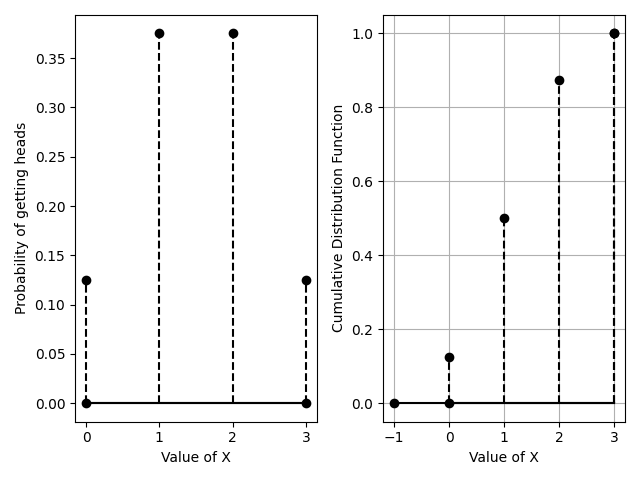
\includegraphics[width=\columnwidth]{/home/sai/Downloads/3(1).png}
 \end{document}